%!TEX root = ../template.tex
%%%%%%%%%%%%%%%%%%%%%%%%%%%%%%%%%%%%%%%%%%%%%%%%%%%%%%%%%%%%%%%%%%%%
%% chapter2.tex
%% NOVA thesis document file
%%
%% Chapter with the template manual
%%%%%%%%%%%%%%%%%%%%%%%%%%%%%%%%%%%%%%%%%%%%%%%%%%%%%%%%%%%%%%%%%%%%

\typeout{NT FILE chapter2.tex}%



\chapter{Literature Review}
\label{cha:LR}

\glsresetall

In this chapter, four main topics will be explored: Mobile Robotics in Smart Agriculture, 
Motion Planning and its Approaches, Robot Control Methods, and Tractor-Trailer-like System Applications, 
as well as an analysis of the results.

\section{Mobile Robotics in Smart Agriculture}
\label{sec:MRSM}
\paragraph{}According to UNESCO, the world population is going to increase by about 30\%
in the next 25 years and with it, the need for food production. To satisfy this need, there will 
have to be an upgrade in agricultural production and to do it, there has been a development of IoT and AI
technologies to help gather information and make better decisions about the crop fields ~\cite{9716089}. 
These technologies acquire data using several sensors, such as humidity sensors, pH sensors, 
temperature sensors and substance level sensors, that communicate wirelessly using a variety 
of case dependant protocols (like ZigBee or LoRa) to make decisions using specific algorithms 
like PID controllers, Time-Controlled algorithms, Fuzzy-Logic or Machine Learning algorithms like neural networks.

\paragraph{}According to ~\cite{robotics10020052, article34} there are also other factors to be considered and those are climate change and the heavy use 
manual labour, which could be scarce if another pandemic or catastrophic event happens, preventing people from working. Agriculture will also 
need to adapt to this, not only using IoT and AI but also using mobile autonomous robots, alone or as a collaborative system. 
These robots are used to perform manual labour tasks (seeding, planting, harvesting), acquire information 
about the fields through physical sensors or cameras built into the robots, and apply pesticides and disease control.

\paragraph{}To execute most of these tasks like harvesting or seeding, some sort of \gls{UGV}, 
like a tractor, is used. For the execution of other tasks like large area monitoring or the broadcasting 
of pesticides an \gls{UAV}, like a drone, is often used. These autonomous vehicles can handle 
tasks that humans would struggle to do more cheaply and quickly. However, these machines have a limited battery capacity and, 
therefore, need to be designed specifically for the task at hand. For instance, in the case of \gls{UAV}s, 
when covering a large area for monitoring, a lot of battery life is required. To facilitate this, 
the software and overall development of the robot need to be specialized ~\cite{article34, app10103453}.

\paragraph{}Going more in-depth into the design features, there are four main issues to consider: locomotion, sensing, 
planning, and manipulation. Starting with locomotion, there are various types of designs, including wheeled 
robots, flying robots, railed robots, wire-suspended robots, legged robots, and tracked robots which are used, 
for example, in wet environments where wheels might get stuck in the mud. When it comes to sensoring, 
it is also highly dependent on the task at hand. If the goal is to differentiate between two fruits with similar colours, 
a regular digital camera might not suffice, a more sophisticated camera with advanced image processing software may be needed. 
Additionally, some characteristics of the environment change, and therefore, the algorithms used must 
account for factors such as direct sunlight, temperature, and humidity. Moreover, planning is the list of 
decisions the robot has made to complete its task successfully. There are several algorithms used, however, 
the most advanced ones are the sample-based ones which have greater performances. Finally, manipulation is the control of manipulators, 
like robotic arms with grippers, to execute a certain task ~\cite{agriengineering2010010}. The choice of manipulator depends on the task, 
however, some robots have multiple manipulators, called \gls{MIARs}, 
to perform multiple tasks, ~\cite{agriengineering2010010} which reduces the number of robots and costs. Per ~\cite{article34, app10103453} some robots are also programmed 
to be able to perform multi-objective path planning which increases efficiency of movement in complex environments, 
increasing overall efficiency of the robot.

\paragraph{}As an example, in ~\cite{10113871}, a robot was created to compensate the lack of labour caused by the aging of the population of Taiwan. 
The environment characteristics of Penghu, Taiwan, are prone to the overproduction of dragon fruit (Pitaya), and therefore this problem needs 
to be fixed to fight its production. Since the terrain is very shallow and has a poor water retainability, in addition to droughts, the soil 
has become arid which might make a wheeled robot bog down. The choice of locomotion for this robot were the tracks. For sensoring, a 9-axis 
gyroscope, to get the robots deviation, a Webcam (Image Sensor), to get the fruits location, and a Lidar to measure the distance between itself 
and any obstacle in its way. To harvest the fruit, it uses a e-axis robot arm with a gripper end-effector. Finaly, path-planning wise, it uses 
the 2-D SLAM algorithm to generate a pixel map and then the Dijkstra algorithm to calculate the fastest route to the target position. 
The experiments on the field revealed a 97\% harvest success rate meaning the method used by the author is appropriate.

\paragraph{}Another example of a solution is the robot in ~\cite{app12094335}, a platform robot developed to try to compensate for the aging of the South Korea’s 
population which is causing a lack of young labour. The robot was designed to work on a paprika greenhouse with a 3-meter-wide corridor, 
where workers traverse, and 0.5-meter-wide ridge between crops where the robot will operate. The ridges between crops have 
hot water pipping which serve as rails and therefore the robot was designed to be both railed and free driven. Its locomotion system consists 
of a two Wheeled drive kit with two main traction wheels in the middle, and four auxiliary smaller wheels to level the platform. Two in the front and 
two in the back. To move autonomously it incorporated a Lidar, to map the environment, a camera, to detect objects, and an encoder, to get the 
current position of the robot. The chassis was adapted to serve as a vacuum system, a lift table system or as just a manipulator. It had two controllers, 
one for the movement control system and another for the manipulation system. However, only the movement system was tested. This robot was not 
tested in the field, but, passed both the maximum load test (withstood 400Kg with no change of the distance between chassis and ground). 
The autonomous driving had some problems with the steering and network making it not ready to operate, however, it is a good start to solving this agricultural problem.

\section{Motion Planning}
\label{sec:MP}
\paragraph{}Motion planning is of the most important steps to achieve autonomous movement in robots, and there are several methods that can be implemented to achieve this.
The goal is to calculate a path that will get the configuration of the robot from a starting position qstart to a goal configuration qgoal, without colliding 
with any obstacle, and to achieve this there exist several methods.
In ~\cite{tamizi2023review, LIU2023120254}, the methods are divided into two categories, Classical Approaches, which include Cell Decomposition, Roadmapping, Sampling-based, and 
Bio-Inspired approaches, Roadmapping approaches, and the Learning Approaches which are the Supervised learning, Unsupervised learning and Reinforcement Learning based approaches. 
Additionally, according to ~\cite{LIU2023120254}, there are two types of planners, Global and Local planners. Global planning is when a path is planned with prior 
knowledge of the environment, whereas Local planning is when a path is planned reactively as the knowledge of the environment is being acquired in real time. 
Global planners focus on modelling method for the environment and path selection where Local planners focus on using data acquisition devices. 
Both types of planners can use the same approaches for path planning. 
\\
\\
To continue there we'll need some definitions:
\begin{itemize}
   \item C-space (C) are all the possible configurations the robot can have, for example in a robotic arm it is all the angles its joints can be in;
   \item $C_{obs}$ are all the configurations where the robot is in contact with an obstacle;
   \item $C_{free}$ are all the configurations possible for the robot to be in, but not in contact with an obstacle $C_{free}  = C \hspace{0.1cm}\textbackslash U\hspace{0.1cm} C_{obs}$;
\end{itemize}

\subsection{Cell Decomposition approaches}
\label{subsec:CD}
\paragraph{}These approaches are called Grid-based because they divide the C-space into a grid where each centre point of a cell is a node. 
The path is chosen as a sequence of these  nodes using algorithms like Dijkstra’s algorithm or A* for example.
There are three main types of Cell Decomposition approaches, the exact, adaptive and approximate cell decompositions~\cite{PATLE2019582}. 
\subsubsection{Exact Cell Decomposition}
\label{subsubsec:ECD}
\paragraph{}The Exact Cell Decomposition approach divides the C-space into small polygonal elements formed by vertical lines created by every vertex of the obstacles. 
See Figure \ref{fig:ExactCellDecomposition} for visual aid.
\begin{figure}[H]
    \centering
    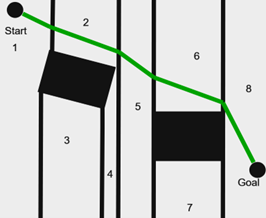
\includegraphics[width=0.5\textwidth]{ECD.png}
    \caption{Exact Cell Decomposition representation; Green line is a possible chosen path}
    \label{fig:ExactCellDecomposition}
\end{figure}
\subsubsection{Adaptive Cell Decomposition}
\label{subsubsec:AdaptCD}
\paragraph{}The Adaptive or Quadtree Cell Decomposition approach firstly divides the C-space into four cells of the same size. Then every cell that is partially occupied will 
keep dividing itself until every cell is either free of obstacles or fully occupied. See Figure \ref{fig:AdaptiveCellDecomposition} for visual aid.
\begin{figure}[H]
    \centering
    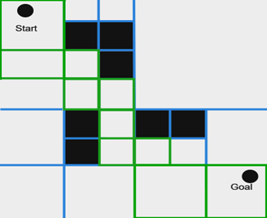
\includegraphics[width=0.5\textwidth]{AdaptCD.png}
    \caption{Adaptive Cell Decomposition representation; Green Squares are the chosen cells/nodes for the shortest path}
    \label{fig:AdaptiveCellDecomposition}
\end{figure}
\subsubsection{Approximate Cell Decomposition}
\label{subsubsec:ApproxCD}
\paragraph{}Finally, the Approximate Cell Decomposition approach simply divides the C-space into a grid with known cell size. The smaller the cells, 
better optimised the path, however, more combinations of path exist making computation more time consuming. There are two types of Approximate Cell Decomposition, 
8-connected and 4-connected where the former accounts for diagonal movement between nodes and the ladder only vertical and horizontal movement. 
See Figure \ref{fig:ApproximateCellDecomposition} for 8-connected.
\begin{figure}[H]
    \centering
    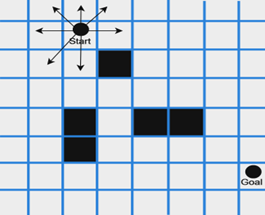
\includegraphics[width=0.5\textwidth]{AproxCD.png}
    \caption{Approximate 8-connected Cell Decomposition representation; Arrows are all represent every possible movement the robot can make}
    \label{fig:ApproximateCellDecomposition}
\end{figure}
\subsection{Grid/Graph Search algorithms}
\label{subsec:GSA}
\paragraph{}Most of the motion planning approaches create graphs or grids where nodes are connected forming paths. After the paths
are created the best one needs to be chosen. To make this choice, graph search algorithms are used. The most common ones 
are the Dijkstra's algorithm and the A* algorithm.
\subsubsection{Dijkstra's Algorithm}
\label{subsubsec:Dijkstra}
\paragraph{}Dijkstra’s algorithm works by looking at the node with the shortest distance to the root of the graph, which
in the beginning is the root itself. Then it calculates the distance to all the nodes connected to the that node (every edge
 has a weight), and then chooses the node with the shortest distance to the root. Every node keeps track of the 
parent node and is updated if a shorter path to said node is found. This process is repeated until
every node is visited. The path is then found by backtracking from the goal node to the root node. 
\begin{figure}[htbp]
    \centering
    \begin{minipage}[b]{0.3\textwidth}
        \centering
        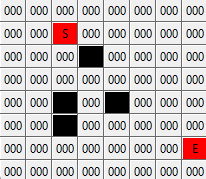
\includegraphics[width=\textwidth]{dijkstraStart.png} % replace with your figure
        \caption*{(a)}
    \end{minipage}
    \begin{minipage}[b]{0.3\textwidth}
        \centering
        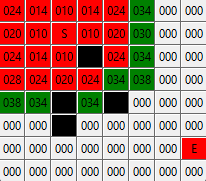
\includegraphics[width=\textwidth]{dijkstraMid.png} % replace with your figure
        \caption*{(b)}
    \end{minipage}
    \begin{minipage}[b]{0.3\textwidth}
        \centering
        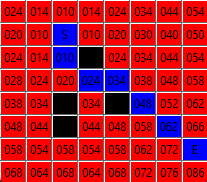
\includegraphics[width=\textwidth]{dijkstraEnd.png} % replace with your figure
        \caption*{(c)}
    \end{minipage}
    \caption{8-connected Dijkstra's Algorithm; a) is the starting C-space; b) is a mid point of the algorithm; c) is the end point of the algorithm; The green squares are the searched neighbours, the red ones are the visited nodes and the blue ones are the chosen path.}
    \label{fig:Dijkstra}
\end{figure}
\subsubsection{A* Algorithm}
\label{subsubsec:A*}
\paragraph{}The A* is similar to the Dijkstra's algorithm, as it also goes from node to node calculating distances, however, 
it has a heuristic function that estimates the distance from the current node to the goal node. The value stored in each node 
instead of being the path distance from the root, is the sum of said distance and the estimated distance towards the goal.
\begin{equation}
    f(n) = g(n) + h(n)
\end{equation}
where $f(n)$ is the value stored in the node, $g(n)$ is the distance from the root to the node, and $h(n)$ is the estimated 
distance from the node to the goal. This way the chosen nodes are biased towards the goal, making the algorithm faster than 
the Dijkstra's.

The algorithm starts in the same way, calculates the $f$ value for all the root adjacent nodes, chooses the smallest value,
and then calculates the $f$ value for all the nodes connected to the chosen node. This process is repeated until the goal 
node is reached. If a value is found that is smaller than the one stored in the node, the value is updated. The path is then 
backtracked from the goal node to the root node.
% make a 3 column figure with 3 pictures
\begin{figure}[htbp]
    \centering
    \begin{minipage}[b]{0.3\textwidth}
        \centering
        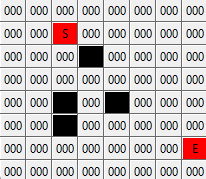
\includegraphics[width=\textwidth]{dijkstraStart.png} % replace with your figure
        \caption*{(a)}
    \end{minipage}
    \begin{minipage}[b]{0.3\textwidth}
        \centering
        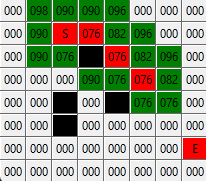
\includegraphics[width=\textwidth]{astarMid.png} % replace with your figure
        \caption*{(b)}
    \end{minipage}
    \begin{minipage}[b]{0.3\textwidth}
        \centering
        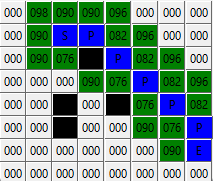
\includegraphics[width=\textwidth]{astarEnd.png} % replace with your figure
        \caption*{(c)}
    \end{minipage}
    \caption{8-connected A* Algorithm; a) is the starting C-space; b) is a mid point of the algorithm; c) is the end point of the algorithm; The green squares are the searched neighbours, the red ones are the visited nodes and the blue ones are the chosen path.}
    \label{fig:A*}
\end{figure}

As seen in Figure \ref{fig:A*}, the path has more diagonal transitions that the one in 
Figure \ref{fig:Dijkstra}, making it slightly longer. This is due to the heuristic function used in the A* algorithm which 
makes it go faster towards the goal, but not always in the shortest path.

\subsection{Artificial Potential Field}
\label{subsec:APF}
\paragraph{}The traditional \gls{APF} approach consists of assigning a positive potential to obstacles and a negative one to the end state. Using the robot as a positive charge, 
the end goal will have an attractive force on the robot while the obstacles a repulsive force. 
This way the robot is attracted to the goal configuration while being repelled by the obstacles. 
This method is advantageous due to its simplicity ~\cite{9830995} and due to its speed when compared to the graph search algorithms ~\cite{100007}. 
However, the main problem with this algorithm is its susceptibility to the local minima problem ~\cite{9830995, 100007}. 
If there is ever a configuration where the repulsive forces generated by the obstacles are symmetrical to the attractive one of the goal state, 
the robot will not be able to move.
\begin{figure}[htbp]
    \centering
    \begin{minipage}[b]{0.45\textwidth}
        \centering
        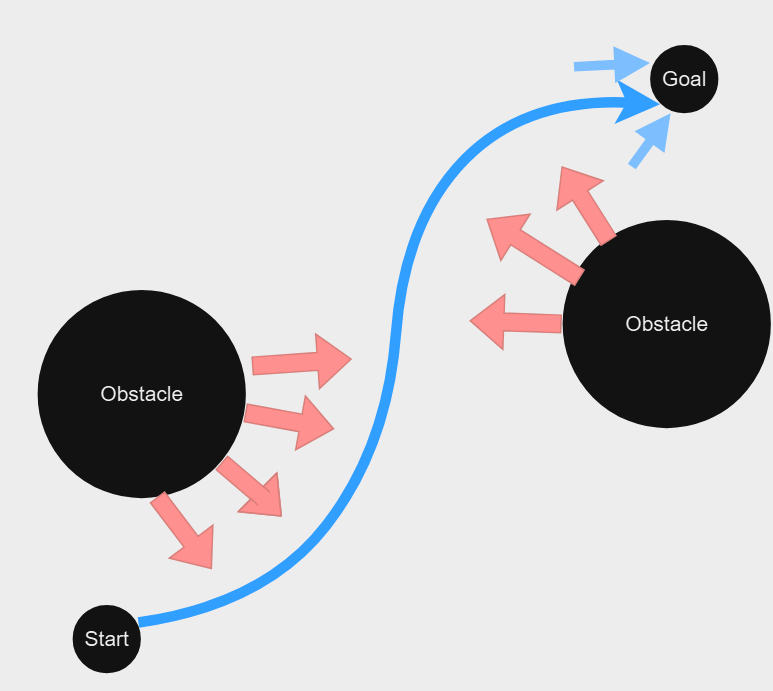
\includegraphics[height=5cm, width=\textwidth]{APF.png} % replace with your figure
    \end{minipage}
    \begin{minipage}[b]{0.45\textwidth}
        \centering
        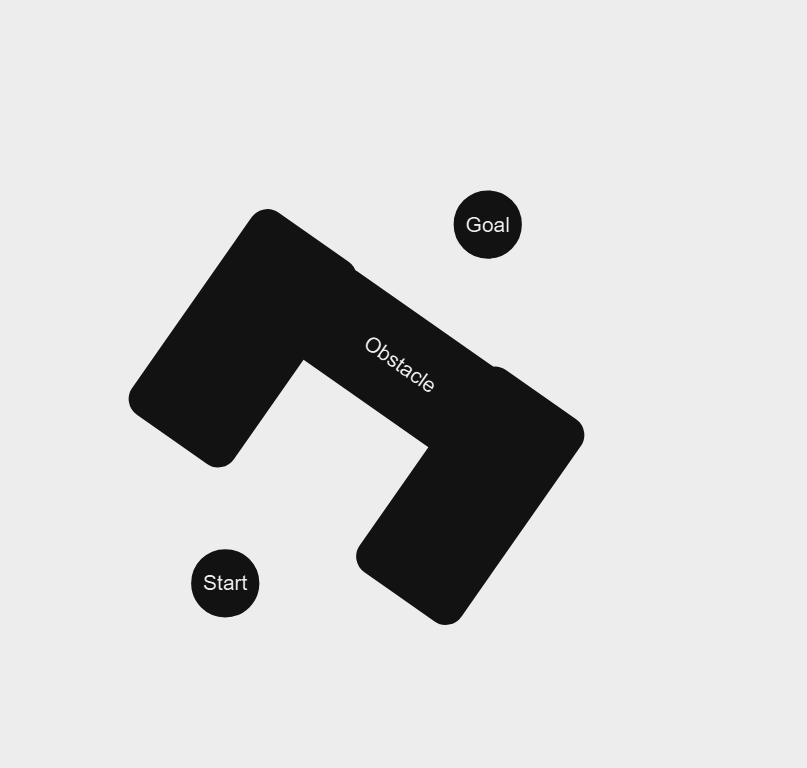
\includegraphics[height=5cm,width=\textwidth]{APFlocalminima.png} % replace with your figure
    \end{minipage}
    \caption{APF algorithm; On the left is the normal functioning of the algorithm where the pink arrows represent obstacle repulsion, the smaller blue ones represent the goal attraction and the curvy blue arrow is the chosen path; On the right is the local minima situation.}
    \label{fig:APF}
\end{figure}

\paragraph{}To solve this local minima problem, the author in ~\cite{9734712} proposed a solution where when the robot is detected to be facing this problem, 
it will move in a random forward direction to get out of that situation. Another approach is to combine multiple methods like the author of ~\cite{8763966} proposed. 
His approach was to use the traditional \gls{APF} until a local minima position is reached and then switches to using the RRT*, a sampling-based algorithm explained in \ref{subsubsec:RRT}, 
to escape it.
\subsection{Sampling-based approaches}
\label{subsec:SB}
\paragraph{}There are two main sampling-based approaches, the \gls{PRM} and the \gls{RRT}. These algorithms sample the C-space
creating nodes and then connecting them forming a roadmap. 

\subsubsection{Probabilistic Road Map}
\label{subsubsec:PRM}
\paragraph{}The \gls{PRM} is divided into two phases, 
being the construction and query phase. The construction phase starts by sampling the $C_{free}$ and establishing feasible or non-obstructed connections between the sampled nodes, 
creating a roadmap R. The query phase joins the initial and goal configurations to the roadmap by connecting them to the closest non-obstructed nodes and then, by using, for example, 
a distance-reduction algorithm like the A* or Dijkstra, obtaining the desired path. 
This approach has difficulty in narrow environments because of its probabilistic nature it is not certain that the sampled nodes can make connections.

\paragraph{}In ~\cite{9286439} this technique is used along with the \gls{APF} approach and the Approximate Cell Decomposition approach creating the HPPRM or 
Hybrid Potential Based Probabilistic Roadmap, to avoid the problem mentioned. It first creates a Potential map with the obstacles’ information, 
then it divides the map into a grid with cells with the same size. Afterwards classifies the cells into High or Low potential depending on the repulsive values calculated. 
Higher potential cells would have more samples than lower potential ones since making connections in the ladder would be easier. After having the nodes, 
the process is the same as the one in \gls{PRM}, connections between nodes are made and then the Dijkstra’s algorithm is used to obtain the shortest path between initial and 
goal configurations.

\subsubsection{Randomly Exploring Random Trees}
\label{subsubsec:RRT}
\paragraph{}The other method, the \gls{RRT}, consists of, with the starting configuration as the root of the tree, randomly sampling the $C_{free}$ and creating a node that 
connects to the nearest one until the end goal is reached. The creation of the node isn’t always on the sample but within a maximum distance in the direction 
to the nearest node. Once the end goal is reached, all needed to do to get the path is to follow the only path from root to goal state. 
Despite always being able to find a feasible path, as samples approach infinity, this method as an issue, since the samples are random, the path created might 
not be optimal in a distance sense. As a solution to this problem, the RRT* algorithm was created. The node creation process is the same as the \gls{RRT}, a sample 
is randomly generated, find the nearest node, create a node within the maximum distance from the nearest node and the sample. The difference is in the 
connection to the tree, instead of connecting it to the nearest node, it searches the nodes around it, within a certain range, and checks if they can be 
rewired so that the paths are shorter. The sampling ends when a short enough path is found, or the number of samples reaches the desired amount. 
There is also another variation of \gls{RRT} which is the bidirectional \gls{RRT} which works exactly like the \gls{RRT} but both goal and stating configurations start 
as a root to a tree, expanding towards each other.

\paragraph{}In ~\cite{9638379}, a combination of variations of the \gls{RRT} are used. The author mentions the use of the Bi-RRT to find, in less time, a 
feasible path between the starting and goal configurations. However, due to the algorithm’s random nature and robot’s constraints, 
the connections between the two trees are made by solving a 2-point Boundary Value Problem which may take too much time in a practical scenario. 
To get around this issue, the author proposed the use of a bidirectional-unidirectional-RRT which functions as a regular Bi-RRT with the two trees growing into each other, 
but, when close enough to connect, it will use a unidirectional search, starting from the initial configuration’s tree, with a bias towards the goal state’s tree.

\subsection{Roadmapping approaches}
\label{subsec:RA}
\paragraph{}The Roadmapping approaches are divided into main two types, the Visibility Graphs and the Voronoi Diagrams which are motion planning approaches
that form connections creating roadmaps. 

\textbf{Note:} The \gls{PRM} and \gls{RRT} approaches weren't included in this section due to their stochastic nature. For the same C-space there
can be multiple roadmaps using PRM and \gls{RRT}, whereas in the Visibility Graph and Voronoi Diagram approaches there is only one.
\subsubsection{Visibility Graph}
\label{subsubsec:VG}
\paragraph{}Visibility graphs function by
representing every object as a polygon and then connecting every adjacent vertex, including starting and end points, 
forming straight lines that do not go through objects. Once multiple connections are formed an optimal path is chosen using an algorithm like A* or 
Dijkstra's. However, this approach has the problem of being time complex and not being dimensionally scalable ~\cite{sym10100450}. 
\paragraph{}An example of the usage of this method can be seen in~\cite{app10165613} where the visibility graph approach is used for in real time
obstacle avoidance for a \gls{UAV}. However, due to mechanical restraints the aircraft needed the connections between edges to be smoother, and therefore
used the Dubin's curves method, which makes a path from A to B using a sequence of straight and curved lined with a minimal R radius imposed
imposed by the necessary restraints ~\cite{aac5c909-7434-3d95-961b-caf3aec6a743}.
Another example of the use of this approach is in ~\cite{LEE2021102887} where the author used the Visibility Graph and the Adaptive or Quadtree Cell Decomposition
methods  to create a path for a marine USV for the coast of South Korea. The map was divided into a grid with four cells, NW, NE, SW, SE, and then would
be divided like explained in \ref{subsec:CD}. After the construction of the quadtree graph, the visibility graph is created using
the nodes in the centre of each cell. The shortest path is then chosen using the Dijkstra's algorithm.
\begin{figure}[h]
    \centering
    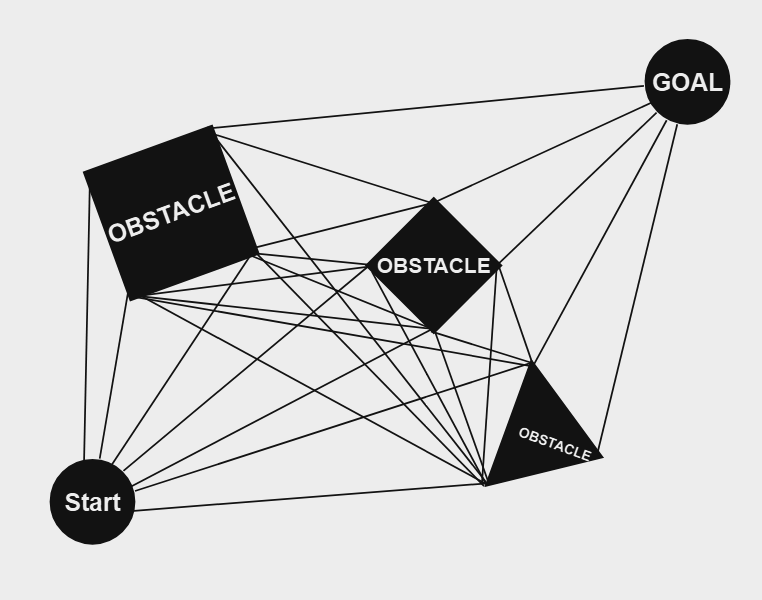
\includegraphics[width=0.5\textwidth]{VG.png}
    \caption{Visibility Graph representation; As explained, the black lines are the connections between the vertices that will then be searched for the shortest path}
    \label{fig:VG}
\end{figure}
\subsubsection{Voronoi Diagram}
\label{subsubsec:VD}
\paragraph{}The Voronoi Diagram consists of two sets, the vertex or node set, and the edge set. The edge set is the collection of all the lines 
which are equidistant to two objects, and the vertex set is the collection of all the points where three or more lines intersect. These objects
may be obstacles or just workspace boundaries. Again, like in the Visibility Graphs, after the diagram is created, the best path can be chosen using
an algorithm like A* or Dijkstra.

\paragraph{}The usage of this approach can be exemplified in ~\cite{8948325} where the author used the Voronoi Diagram along with the RRT* and Potential Field
approaches to create a path for a \gls{UGV} in a indoors environment. Firstly, the planner would create a Voronoi Diagram of the C-space, however This
would not suffice for a successful path plan due to the robots mechanical constraints. For this, a potential function was used to create a map
where the most attractive points would be in the path chosen using the Voronoi Diagram. Afterwards, the RRT* algorithm was used to create the
optimal path sampling with a bias towards the attractive field. Despite this approach being successful in most cases, there were still cases where
the robot's dynamics would prevent it from following the desired path. The author then suggests that this problem would easily be overcome by
making a circle around the robot and if the circle isn't able to move in that position, the position would be discarded, and another path would be chosen
in the Voronoi Diagram phase.
\begin{figure}
    \centering
    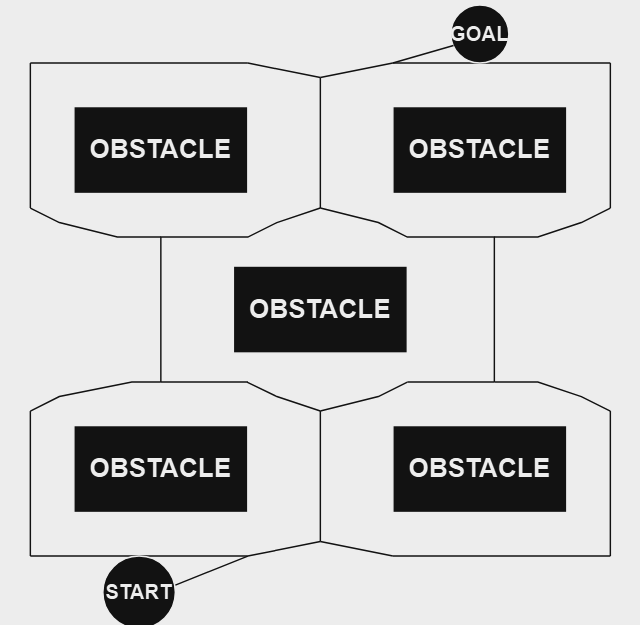
\includegraphics[width=0.5\textwidth]{VoronoiG.png}
    \caption{Voronoi Diagram representation; The black lines keep the same distance to the obstacles and the map edges}
    \label{fig:VoronoiG}
\end{figure}

\subsection{Bio-Inspired approaches}
\label{subsec:BI}
\paragraph{}The Bio-Inspired approaches are, as the name would suggest, inspired by natural systems. The main methods are the \gls{ACO},
\gls{PSO} and the \gls{GA}. These optimization algorithms minimize a specific
Objective or Cost function, which could factor path length, energy spent, or any other example specific characteristic
that could impact performance ~\cite{s23063051}. 
\subsubsection{Particle Swarm Optimization}
\label{subsubsec:PSO}
\paragraph{}The \gls{PSO} algorithm starts by creating a swarm of particles, each with a position and velocity. In the motion planning context,
each particle represents a possible solution or, in other words, a feasible path. The particles' position and velocity are updated, with each iteration, according to 
the following equations:
\begin{equation}
    v_{i}^{t+1} = wv_{i}^{t} + c_{1}r_{1}(pbest_{i} - x_{i}^{t}) + c_{2}r_{2}(gbest - x_{i}^{t})
\end{equation}
\begin{equation}
    x_{i}^{t+1} = x_{i}^{t} + v_{i}^{t+1}
\end{equation}
where $v_{i}^{t}$ is the velocity of particle i at time t, $w$ is the inertia weight, $c_{1}$ and $c_{2}$ are the cognitive and social coefficients,
$r_{1}$ and $r_{2}$ and randomly generated values between 0 and 1, $pbest_{i}$ is the best position of particle i, and $gbest$ is the best position of the swarm.
The algorithm stops when a maximum amount of iterations K is reached.
\paragraph{}This approach was used in ~\cite{4178249} the author defined the particles as a set of parameters of cubic splines, which would connect to form
a smooth path for the robot. The cost function used considered the path length, the minimum distance between the robot and
the closest obstacle, and the Euclidean distance between the robot and the goal configuration. This method was compared to the
visibility graph and the \gls{APF} and found that it was able to find a smoother and more easily executable path (less discontinuities)
while maintaining a short path distance. Due to how slow the algorithm is, the author says that it can only be used in a static
environment.
\subsubsection{Ant Colony Optimization}
\label{subsubsec:ACO}
\paragraph{}The \gls{ACO} algorithm is inspired by the behaviour of ants when looking for food.
When traveling, ants leave pheromone trails so the other ants can follow them. The algorithm tries to mimic this behaviour
by creating a set of artificial ants that will create a path from the starting to the goal configuration. The probability of
a $k$ ant of going from node $i$ to node $j$ at time $t$ is given by the following equation:
\begin{equation}
    P^k_{ij} = \frac{\tau_{ij}^{\alpha}(t)\eta_{ij}^{\beta}(t)}{\sum_{k \in N_{i}}\tau_{ik}^{\alpha}(t)\eta_{ik}^{\beta}(t)}
\end{equation}
where $N$ is the set of nodes connected to $i$, $\tau$ is the pheromone level of the path from $i$ to $j$, $\eta$ is the heuristic information or 
proximity, $\alpha$ is the pheromone incentive factor which means that the larger the $\alpha$ the more wight the pheromone level has
on the probability of a path being chosen, and $\beta$ which acts the same way as the precious coefficient only not for pheromone level
but for proximity between nodes ~\cite{aocet1}. The pheromone level is updated at the end of each iteration using the following equation:
\begin{equation}
    \tau_{ij}(t+1) = (1 - \rho)\tau_{ij}(t) + \rho\Delta\tau_{ij}(t)
\end{equation}
where $\rho$ is the pheromone evaporation rate and $\Delta\tau_{ij}$ is the increment amount of pheromone left by the ants in the path from $i$ to $j$.
Given a maximum number of iterations, naturally the shortest path will be the one with the most pheromone left by the ants.
Due to its robustness, global optimization ability, and possibly being used in combination with different heuristic 
algorithms, the \gls{ACO} is widely used in path planning. However, in complex environments, the algorithm may get stuck in a local minima or get into a 
Deadlock state where the ants can't escape from a specific node as there are not any not explored ones nearby ~\cite{aocet2}.

\paragraph{}In ~\cite{XIE2022104076} the author proposes an improvement to the \gls{ACO} algorithm to plan a path in a radioactive environment. 
The proposed method added a chaos optimization algorithm to create initial random initial paths, it changed the pheromone
update equation to include radiation level as a negative trait and also added a local search optimization to avoid the local minima problem. 
This method proved to be more efficient than the traditional \gls{ACO} and \gls{PSO} algorithms in the same scenario. 
\subsubsection{Genetic Algorithm}
\label{subsubsec:GA}
\paragraph{}This method is inspired on the evolution of species. The algorithm starts by creating a random population of chromosomes, each representing a 
possible solution to the problem, like in the \gls{PSO}. With every iteration each chromosome is evaluated using a 
fitness function, which is the cost function in the motion planning context. The better performing chromosomes have increased
changes of being selected for reproduction. The reproduction process is done by selecting two chromosomes and crossing them over, creating
a new chromosome. This new chromosome can be mutated in order to create different solutions and therefore diversity. The process is repeated until a maximum amount of iterations
is reached or a desired fitness level is achieved.
\paragraph{}An improved version of this method was used in ~\cite{guo2019optimal} to plan a path for an Unmanned Surface Vehicle. The 
chromosome encoding was done using sets of angles and velocities ($\theta$, $v$) creating one hour steps. In the traditional
GA, mutation is done by replacing a parent gene with a random value. The author believes that this 
approach is not optimal suggesting an alteration to the formula by taking the previous value and adding a 
value dependant on the gene's position multiplied by a random value and a constant. This change in the approach
makes it so the mutated child will be closer to the parent, making convergence faster. The fitness function used
is a Monte Carlo approximation of the cumulative detection probability which calculates the 
efficiency of a path. This method showed better results than the traditional \gls{GA} as it had faster convergence
to the optimal value and was also faster.
\subsection{Learning-based approaches}
\label{subsec:LB}
\paragraph{}There are three main types of learning based approaches, Supervised, Unsupervised and Reinforcement learning ~\cite{MLT1}.
\subsubsection{Supervised Learning}
\label{subsubsec:SL}
\paragraph{}The Supervised Learning methods, like most ML approaches, are used to predict a value based on a trained model. To train this model
a labelled and classified dataset is needed. The model is then trained based on the provided data and is used as necessary. The most 
commonly used Supervised Learning methods are the artificial neural networks, and the \gls{SVM}, however, 
methods can be used like linear regressions, randomforest, logistic regressions, convolutional neural networks, recurrent 
neural networks, K-nearest neighbour, and Naïve Bayes ~\cite{MLT1}.
\subsubsection{Unsupervised Learning}
\label{subsubsec:USL}
\paragraph{}The Unsupervised Learning methods function similarly to the Supervised Learning methods, however, 
there is no labelling or classification of the datasets. The models are trained to find clusters or patterns in the data ~\cite{USLT}.
Due to this difference the dataset usually needs to be larger than the one used in Supervised Learning methods ~\cite{MLT1}.
\subsubsection{Reinforcement Learning}
\label{subsubsec:RL}
\paragraph{}The Reinforcement Learning methods, much like the unsupervised ones, do not get a labelled or classified dataset to be trained 
on. Instead the model is trained by trial and error, where the model is rewarded or punished based on the arrived state ~\cite{RLT}.

\paragraph{}Examples of the usage of Learning-based approaches can be found in~\cite{RLEX1} where the author used a Reinforcement 
Learning approach to generate actions the robot should take to reach the desired configuration. Another example can be found in 
~\cite{MLEX2} where the author proposed a new method combining Convolutional Neural Networks and the RRT* algorithm, and concluded
 that the new method outperformed the conventional RRT* algorithm in the same scenario.

\section{Motion Control}
\label{sec:MC}
\paragraph{}With a path calculated, the next step is to make the robot follow it, for this we use a robot controller or path tracker. In this section,
 the most common path tracking controllers will be explored, and these controllers are the \gls{PP}, the \gls{MPC}, and the \gls{DWA} ~\cite{macenski2023regulated}.

\subsection{Pure Pursuit}
\label{subsec:PP}
\paragraph{}The algorithm works by calculating an arc between the robot's nearest waypoint and the one that is at least a 
lookahead distance L away ~\cite{macenski2023regulated}. Assuming the Path as a set of waypoints $P = {p_0,p_1, p_2, ..., p_n}$, the point nearest to the robot is chosen 
as $p_r$ and the lookahead point $p_l$ is chosen as follows:
\begin{equation}
    dist(p_i) = \sqrt{(x_r - x_i)^2 + (y_r - y_i)^2}
\end{equation}
\begin{equation}
    p_l = p_i \in \mathcal{P}_t, \quad
    \begin{cases}
        dist(p_{i-1}) < L \\
        dist(p_i) \geq L
    \end{cases}
\end{equation}
with a chosen $p_l$ it is now possible to calculate the curvature of the arc that will be followed by the robot:
\begin{equation}
    \kappa = \frac{2y_l'}{L^2}
\end{equation}
where $y_l'$ is the lookahead's point lateral coordinate and L the desired distance between the robot's point and $p_l$. 
This algorithm assumes a constant velocity and lookahead distances and, therefore, to improve performance in more 
complex scenarios, a new version of this controller was created, the Adaptive Pure Pursuit, where  
the lookahead distance is proportional to the current velocity:
\begin{equation}
    L_t = v_t \cdot l_t
\end{equation}
where $L_t$ is the lookahead distance at time t, $v_t$ is the current velocity, and $l_t$ is the lookahead gain.
\subsection{Model Predictive Controller}
\label{subsec:MPC}
\paragraph{}The \gls{MPC} is a control method that uses the model of the robot system to optimize 
a cost function. The controller works by, given an Horizon N, predicting the future states of the robot and then minimizing
 the cost function to obtain the optimal control inputs for the states in the horizon. The controller keeps iterating 
this process, predicting the future states and optimizing control action until the goal configuration is reached.

The cost function will vary from case to case but in a path tracking problem can be defined as ~\cite{MPCcost}:
\begin{equation}
    J(\Delta \mathbf{U}, \mathbf{e}) = \frac{1}{2} \left\{ \sum_{i=k+1}^{k+N_p} \|\mathbf{e}(t_i)\|_{\mathbf{Q}}^2 + \sum_{i=k+1}^{k+N_c} \|\Delta \mathbf{u}_e(t_i)\|_{\mathbf{R}}^2 \right\}
\end{equation}
where $e(t_i)$ is the error between the reference point and the robot's current position, $\Delta u_e(t_i)$ is the increment of the control input, the 
$N_p$ and $N_c$ are the prediction and control horizons, and $Q$ and $R$ are the weighting matrices for the error and control input increment, respectively. 
Additionally, the control action can be constrained by the robot's physical limitations, like maximum and minimum velocity, acceleration, and jerk.

\subsection{Dynamic Windows Approach}
\label{subsec:DWA}
\paragraph{}The \gls{DWA} works by, like in the \gls{PP}, creating arcs the robot will follow. Firstly, it generates 
circular trajectories with different pairs of velocities and angular velocities. Then it chooses 
the only pairs which allows the robot to stop before reaching an obstacle. Finally, it applies the 
dynamic window where it eliminates the pairs in which the required velocities aren't reachable in the 
chosen time period. After eliminating all the non usable pairs, the pair with the smallest value 
when the cost function is applied is chosen as the control action ~\cite{DWAT}. The cost function can be defined as:
\begin{equation}
    J(v, w) = \alpha \cdot \text{heading}(v, w) + \beta \cdot \text{distance} + \gamma \cdot v
\end{equation}
where $\alpha$, $\beta$, and $\gamma$ are the weighting factors, the heading is cost of the difference between where the robot 
is facing and the desired node direction, the distance is cost of the distance between the robot and the closest obstacle, and v is the
 robot's velocity. This process is repeated between nodes until the goal configuration is reached.

\section{Related Work}
\label{sec:TTS}
\paragraph{}Since the system that this thesis will be focusing on is a tractor-trailer system, 
in this section there will be a brief explanation of the system and some ways its been approached.

\subsection{System Description}
\label{subsec:SD}
\paragraph{}The tractor-trailer system is a system where a self-propelled vehicle, the tractor, pulls a 
non-propelled vehicle, the trailer. This system has been modelled in many papers and generally takes the 
following form ~\cite{theman, ttdynamics2}:
\begin{equation}
    \dot{x} = v \cos(\theta_0)
\end{equation}
\begin{equation}
    \dot{y} = v \sin(\theta_0)
\end{equation}
\begin{equation}
    \dot{\theta_0} = \frac{v}{WB}tan(\phi)
\end{equation}
\begin{equation}
    \dot{\theta_1} = \frac{v}{RTR}sen(\theta_0-\theta_1)
\end{equation}
where $x$ and $y$ are the hitch position, $v$ is the robot's velocity, 
$\theta_0$ is the tractor's orientation, $\theta_1$ is the orientation of the trailer, $\phi$ is the 
steering angle, and WB and RTR are the are the wheel base distance (distance between axles) 
and the distance between the hitch and the trailer's rear axle, respectively.

\subsection{Applications}
\label{subsec:APP}
\paragraph{}Some applications of the tractor-trailer system can be found in ~\cite{theman}, 
where the author proposed a Voronoi Hybrid A* for the path-planner and two pure-pursuit controllers 
as path trackers. The author concluded that the traditional approaches were not feasible due 
to generating paths that wouldn't account for the trailer's non-holomic constraints. Therefore, 
a different version of the A* was used. The Hybrid A* is much like the traditional one, however, 
instead of only being able to move to the nodes or grid cells, the nodes generated in the Hybrid A* 
contain the robots dynamics $(x,y,\theta_0,\theta_1,d)$ where $d$ is the direction of motion of said 
node (forward or reverse), and can reach anywhere in the continuous state space. The cost of each 
node is calculated penalizes the change of direction, backwards movement, steering input, change of 
steering input, jack-knifing and path length. Since these nodes have discrete values, it is not 
possible to always reach the desired nodes, therefore, the author used a Dubin's curve to connect 
waypoints generated by a traditional A* search on the Voronoi Graph. This approach was compared to the Hybrid A* without 
the Voronoi Graphs and the Voronoi Hybrid A* was able to create slightly shorter paths a thousand times 
faster. With a generated path, the author used two pure pursuit controllers that switched depending on the 
direction $d$ of a node. This approach to the tractor-trailer problem was able to manoeuvre in 
tight indoor environments which is a necessary feature in the context of this thesis since greenhouse 
and farm corridors are typically narrow. This approach is also successful because it takes a relatively 
short time to generate a smooth path, however, it does not include a local planner for dynamic environments which 
may be crucial in a real-world scenario where workers or other robots may be present.

\paragraph{}Another application of the tractor-trailer system can be found in ~\cite{mpconly}
where the author created a path tracker using an mpc controller. The systems model is slightly different 
from the previous as the author used both the translational velocity and the angular velocity as control 
inputs $u^T=[v, w]$. The system's dynamics become the following:
\begin{equation}
    \dot{x_1} = v \cos(\theta_0)
\end{equation}
\begin{equation}
    \dot{y_1} = v \sin(\theta_0)
\end{equation}
\begin{equation}
    \dot{\theta_0} = w
\end{equation}
\begin{equation}
    \dot{\theta_1} = -v\frac{1}{l_2}sin(\theta_1-\theta_0)  + w\frac{l_1}{l_2}cos(\theta_1-\theta_0)
\end{equation}
where $x_1$ and $y_1$ are the tractors centre position, $l_1$ is the distance between the tractor's front axle and the hitch, 
and $l_2$ is the distance between the hitch and the trailer's rear axle.

The obstacles, walls and the robot were expressed as polygons to facilitate the collision avoidance as 
this approach has no path planner, only a few hand placed waypoints. With these polygons, the 
Farkas' lemma to create a constraint for the mpc controller by expressing the polygons as two matrices
$A$ and $b$ to discritise the obstacles position and orientation.

The cost function created took into consideration the deviation from the goal state, the deviation 
from the reference translational velocity and the variation of input control:
\begin{equation}
    J = x_e^{goal}(N)^TSx_e^{goal}(N) + (\sum_{i=0}^{N-1}  x_e^{goal}(k)^T Q_1 x_e^{goal}(k) + {v_1}_e^{ref}(k)^T Q_2 {v_1}_e^{ref}(k) + \Delta \hat{u}^T(k)Q_3\Delta\hat{u}(k)) \Delta \tau
\end{equation}

where $x_e^{goal}$ is the error between the goal state and the current state, ${v_1}_e^{ref}$ is the error between the current velocity and the 
reference velocity, $\Delta \hat{u}$ is the control input increment, and $\Delta \tau$ is the time step. 
The controller was constrained by the robot's physical limitations in $u^min$ and $u^max$ and the obstacle avoidance equation. 
This cost function is minimised in every iteration until the horizon N is reached.

This approach to path tracking was tested using a narrow environment with four waypoints that would 
appear one by ne as the robot reached them. The testing occurred in two phases, one being in a static 
environment and the other in a dynamic one. In the first one the robot was able to reach the 
goal while managing tight curves and counter curves. However, in the second phase, the robot 
encountered a problem when the dynamic obstacle was placed in front of the robot, as the robot couldn't 
avoid it and had to reverse to avoid a collision. This happened because the obstacle wasn't considered 
dynamic by the model and couldn't predict its movement.

Overall, this approach was able to reach the waypoints without collisions and is very promising, however, 
it does not have a path planner to place the waypoints and has to be done by hand. It starts to 
tackle the object avoidance issue to some successful extent but could be improved.

\paragraph{} In ~\cite{ttex3} an exact local planner was used to solve this problem. The tractor-trailer is a 
non-holomic system that can't be integrated, however, if the steering angle and velocity were constant, 
the system would now be integrable. The author used this concept to create rotational and translational 
paths for this system. Since the steering angle is constant and constrained by the vehicles dynamics 
it was possible to calculate the angle for each arc by using the following equation:
\begin{equation}
    \phi = -arctan(\frac{L_1sin(\theta_1)}{L_2})
\end{equation}
where $L_1$ is the distance between the hitch and the tractor's front axle, $L_2$ is the distance between the 
hitch and the trailer's rear axle, and $\theta_1$ is the orientation of the trailer. This approach 
resembles a \gls{PP} as it also calculates the curvature of the arc needed for a smooth 
path. The paths between two nodes are created by connecting two rotational paths and one translational path, this means, two arcs around 
the nodes and one straight line connecting them. The author mentions that this method can't deal 
with obstacle avoidance, however, if a global planner was integrated, this wouldn't be 
a problem since the nodes would be place in a way that connections would be collision free. 
The testing revealed that this approach could generate a feasible and smooth path in under two seconds, 
which for the time (1995) was quite a fast time. This approach wouldn't suffice for this thesis' 
problem as a whole, however could be used as a path tracker instead of a path planner.

\section{State of the art Summary}
\paragraph{}To summarize, the tractor-trailer pesticide spraying robot proposed in this dissertation 
could be of help in the agriculture industry, and, to develop this project there are several 
approaches to be considered. When it comes to path planning, the Hybrid A* algorithm is a 
good choice as its nodes take into account the robot's dynamics, this algorithm could be used 
in combination with the Voronoi Graphs to create a faster path, like in \cite{theman}. To 
control the robot, the most used option would be the \gls{MPC}, as it can predict 
future states and optimize the tracking problem, however, this approach could be overkill if the path 
is already calculated. The next best option would be the \gls{PP}, as it is simple and can reduce the tractor-trailer problem into 
just a car problem by having steering and velocity as constant values. For a local planner, in case 
a dynamic object appears in front of the robot, the \gls{MPC} could now be used to reach the next node in the path, 
as it could take too much time for a complete replan of the path. 

This project is a very important one, as there isn't a lot of documentation on solutions for this problem, and 
especially in the context of Smart Agriculture.
